% ------------------------------------------------------------------------------
% Chapter 7 : Results
% ------------------------------------------------------------------------------
\setlength{\parindent}{4em}
\setlength{\parskip}{1em}

In this chapter, we are going to see results using prediction framework. Training data collected for single core, dual core with no load and dual core with full load using training framework. We saw intermediate results for performance measurement tools, results from data analysis techniques. But to make prediction of the software or application executing on hardware platform, we are going to select one of the learning algorithm between CLSLR, Lasso and Ridge regression from previous chapter.  We are going to use training data to learn the mapping and predict the results for new application which is not included during the collection of training data. We are going to use application from MiBench benchmark suite to test the prediction accuracy of the results. But before that we need to select the algorithm. 

\section{Cross Validation}
There are needs to check or validate the stability of learning model, assurance of model has got most of the patterns from data correct and model is not picking the noise. This is the process of validation where it checks the relationship between variables are acceptable as description of data, and it is known as cross validation in field of machine learning. In basic term of cross validation, training data is divided into two parts one is intermediate training data and second is test data.  Intermediate training data is applied to machine learning algorithm to learn the relationship and then test data is applied to check the accuracy of the results. This techniques helps to tune the learning model get the more accurate results and then can be applied to real projects or scenarios. Cross validation provides the fine tunning of the model.

\par in this thesis work, we are using 10 fold cross validation technique. Above paragraph we mentioned general cross validation technique which is also known as Holdout method. Disadvantage of this method is that some portion of the training data is lost in test part. To overcome this issue of losing the data, K-fold cross validation is used. In K-Fold cross validation techniques, data is divided into K subsets. In our case we are using 10 Fold method that means our training data is divided into 10 subsets. Now Holdout method is applied in iterative manner. Each time one of the \textit{k} subset is used as test set or validation set and other \textit{k}-1 subsets are put together to form intermediate training data. This process runs iteratively for 10 times and error estimation is averaged over all \textit{k} trials to get effectiveness of model. This method avoid the losing of the data and laso reduces the bias and variance of data significantly to avoid overfitting of the data. 

\par Followings the results of the cross validation techniques used on lasso and ridge regression algorithm.  We were not able to apply cross validation results on CLSLR because as compared to lasso and ridge algorithm, CLSLR is too slow to calculate the results.  It uses neighborhood technique and perform optimization everytime.  So to apply K fold cross validation, where data iteratively tested in 10 subsets was taking more than weeks to collect the results.  We also tried other options but due technical difficulties such as regular security update from company caused restart of the system, which resulted in that we were not able to get enough computing time to check the cross validation results for CLSLR algorithm. 

\begin{figure}[h!]
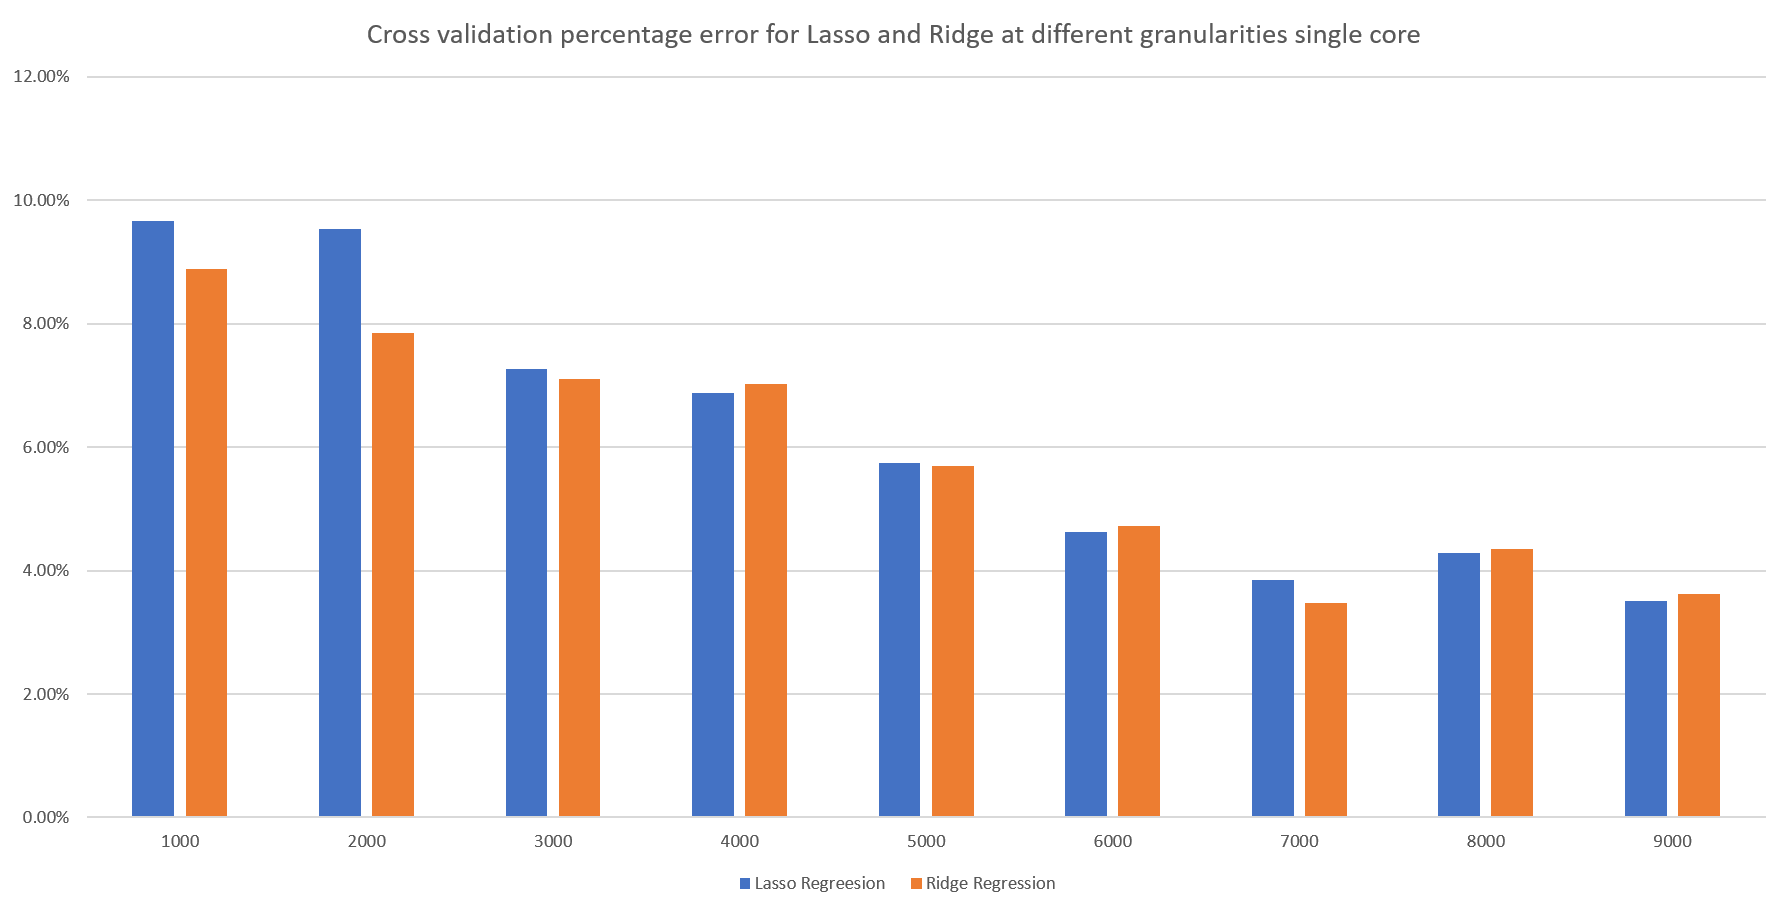
\includegraphics[width=12cm, height=8cm]{./images/CV_single_core}
\centering
\caption{Cross validation results for single core}
\label{fig:training}
\end{figure}

\begin{figure}[h!]
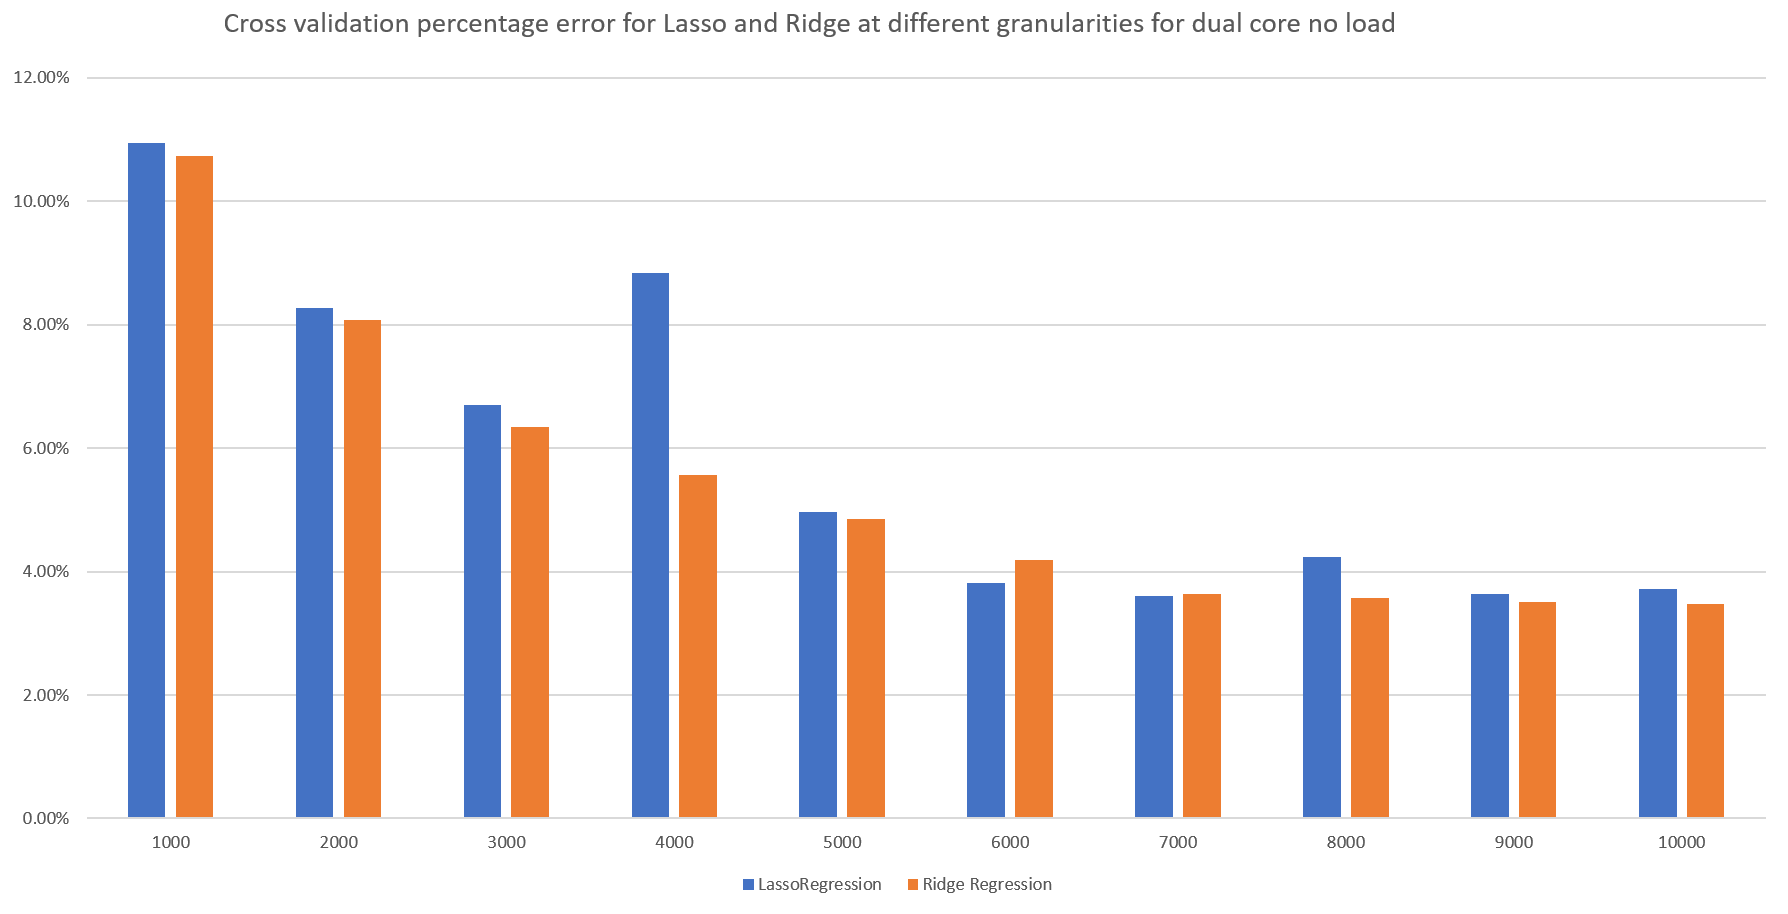
\includegraphics[width=12cm, height=8cm]{./images/cv_no_load}
\centering
\caption{Cross validation results for dual core no load}
\label{fig:training}
\end{figure}

\begin{figure}[h!]
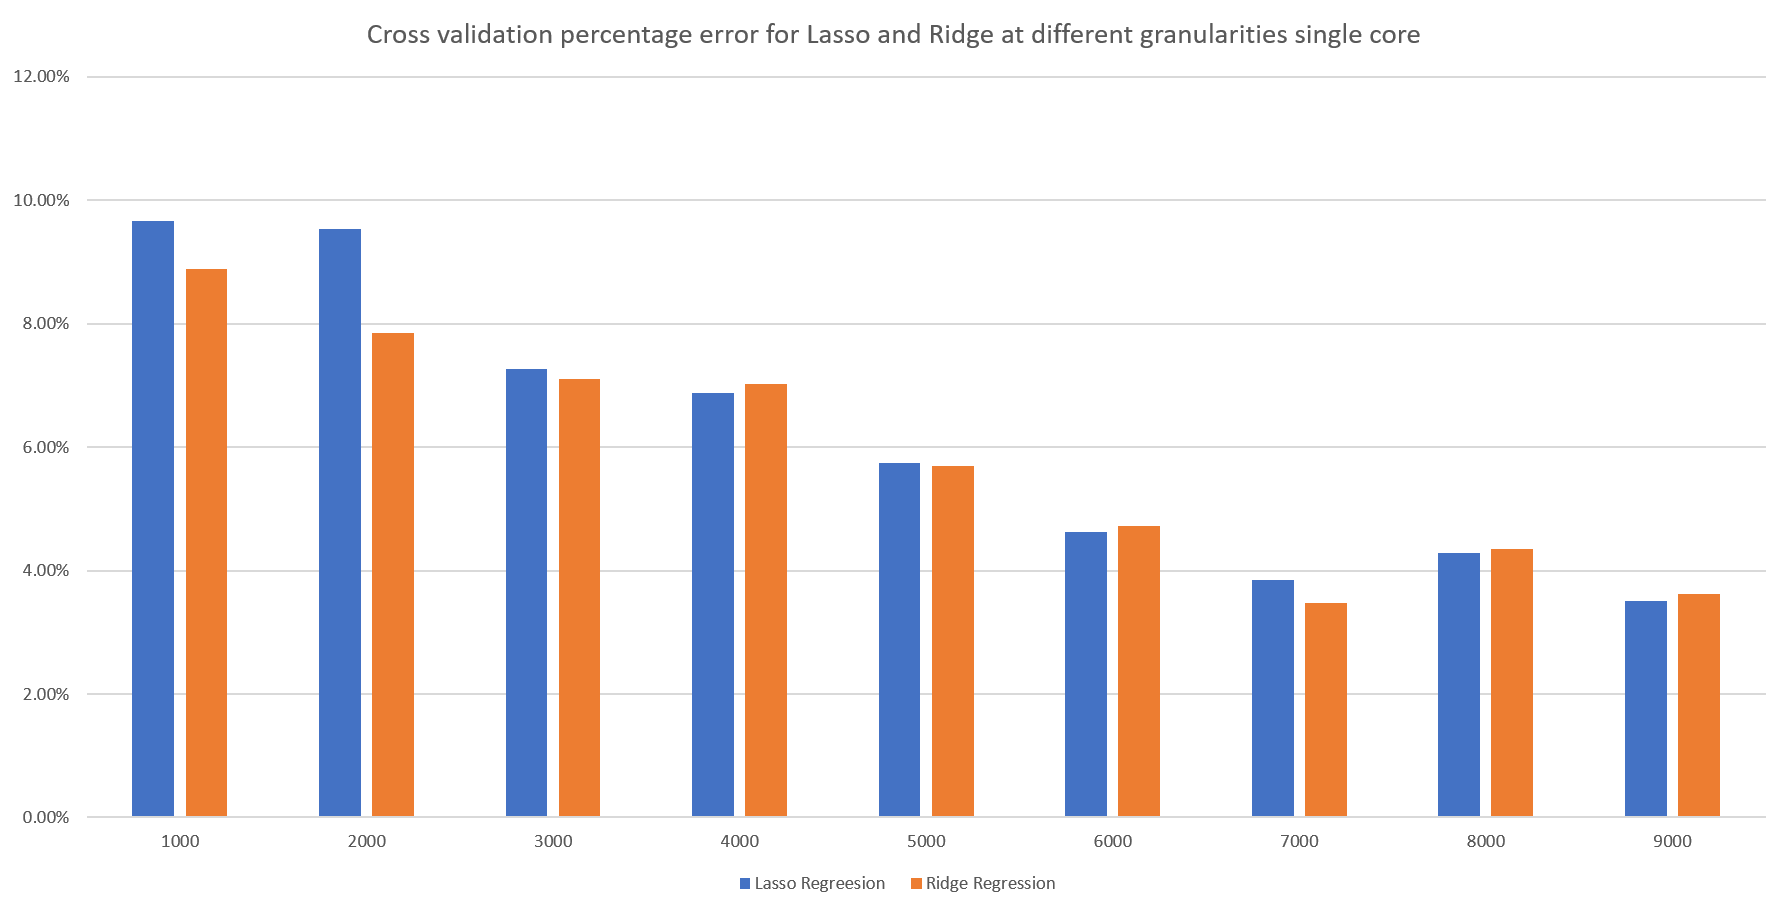
\includegraphics[width=12cm, height=8cm]{./images/CV_single_core}
\centering
\caption{Cross validation results for dual core full load}
\label{fig:training}
\end{figure}

\par We can see in the results that as granularity increases the cross validation results also changes that means at medium granularities accuracy is more. Also there is not much difference between cross validation error of lasso and ridge regression. Both are showing similar results with smaller change in values.  So we are going to use both  to test the prediction accuracy on new programs. 

\section{Response time}
Response time is time require to predict the results. We are goigng to compare the response time of CLSLR, lasso and ridge algorithms. Response time measured prediction of 1000 inputs and measured in seconds.  Following diagram illustrate the response time, 
\begin{figure}[h!]
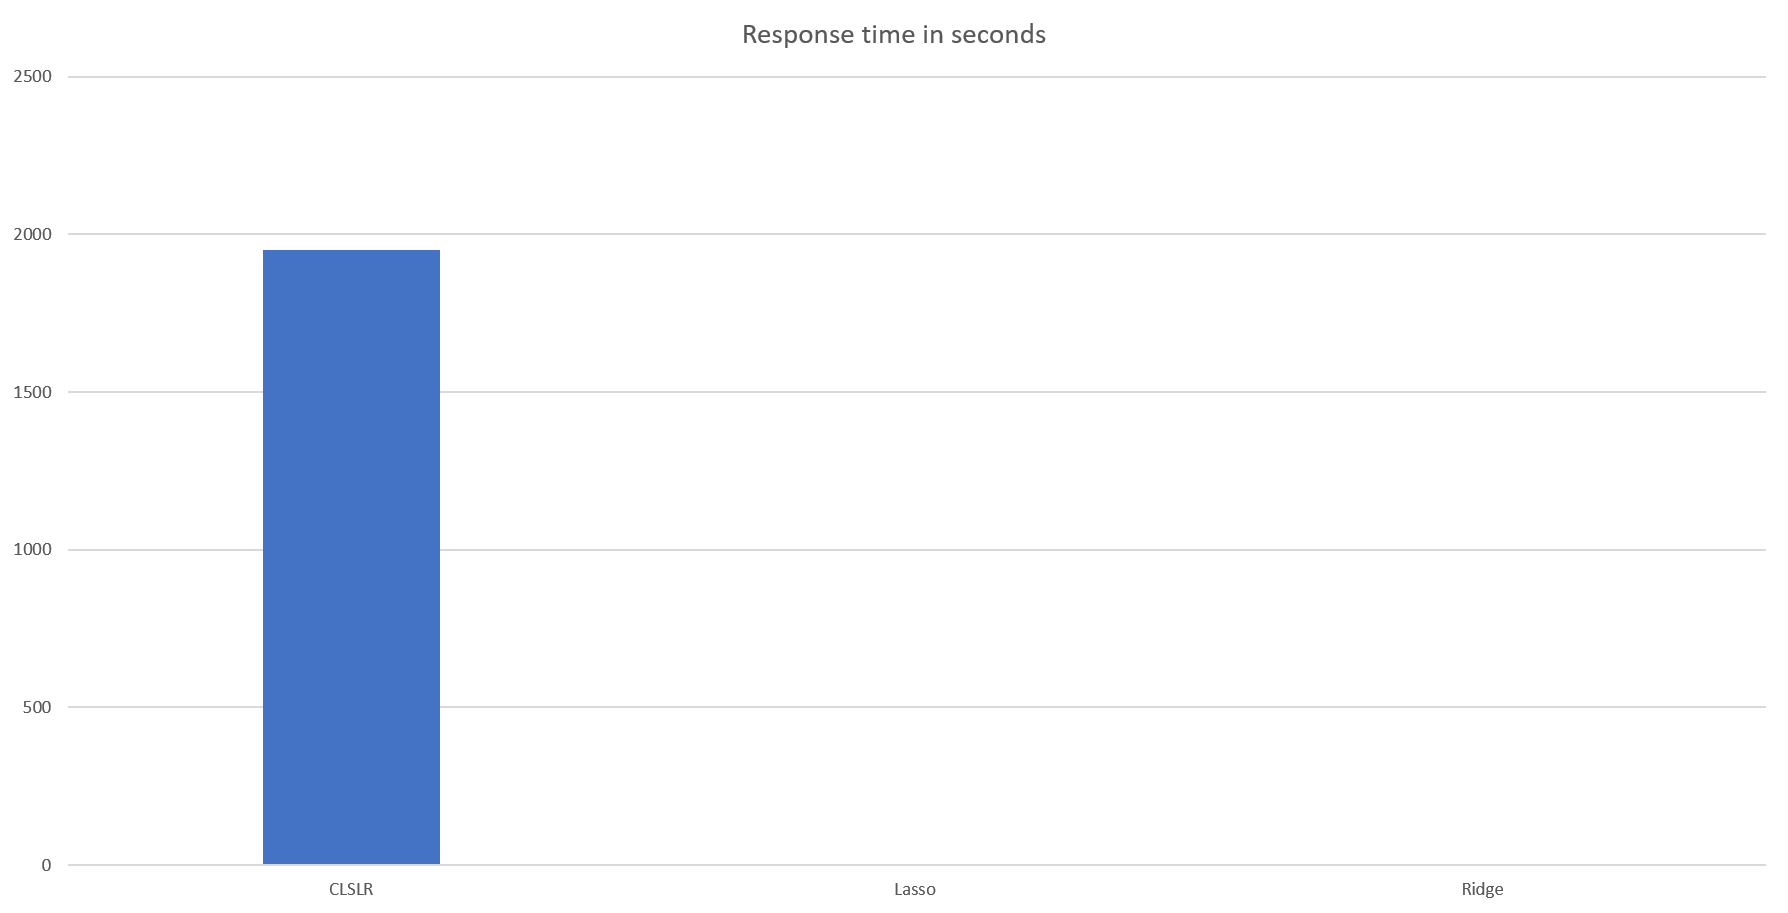
\includegraphics[width=10cm, height=6cm]{./images/response}
\centering
\caption{Response time for algorithms}
\label{fig:training}
\end{figure}

As we can see to predict 1000 inputs, CLSLR taking 1951 seconds, approximately 2 seconds for each input. It is because it perform optimization for each input by finding nearest neighbors to it which is time consuming process. Unlike CLSLR, rigde and lasso take milliseconds to predict the output for same size of input. We can conclude here that CLSLR is slow algorithm as compared to other two algorithms. 

\section{Prediction Accuracy}
To test accuracy of lasso and ridge, we are going to predict the performance of MiBench benchmark suite using lasso and ridge algorithms. We are going to predict the performance of basicmath, bitcount, qsort, dijkstra, patricia, strinsearch, sha, crc32 and fft. These programs are never used to collect training data. We are going to predict the number of cycles for these programs. We predicted the results for single core, dual core without load and dual with load. 

\subsection{Single Core}
Following figure \ref{fig:r_single} shows the prediction average accuracy error in percentage for all application at granularity of 6000 on single core. Both training data and input data of applications are collected at granularity of 6000 o single core. 

\begin{figure}[h!]
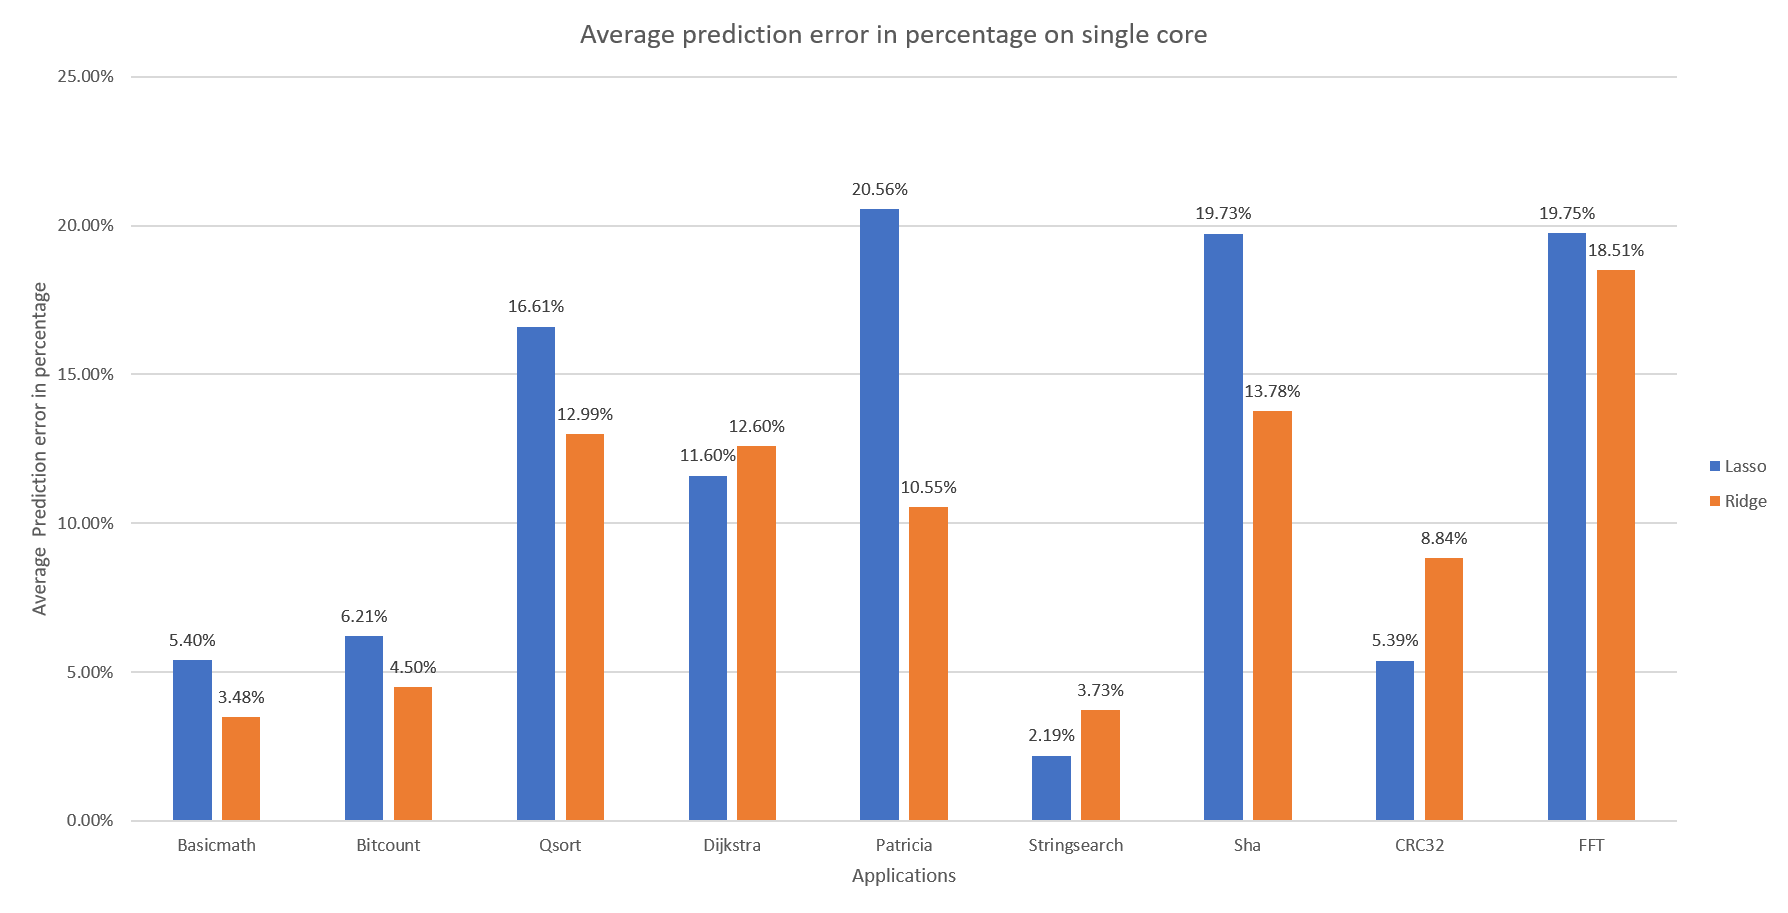
\includegraphics[width=12cm, height=8cm]{./images/result_single}
\centering
\caption{Prediction results collected at granularity of 6000 for single core}
\label{fig:r_single}
\end{figure}

\subsection{Dual Core without Load}
Following results in figure \ref{fig:r_dual_no} are for prediction accuracy on applications on dual core without load at granularity of 8000. Both training data and input data of applications are collected on dual core without load at granularity of 8000. 

\begin{figure}[h!]
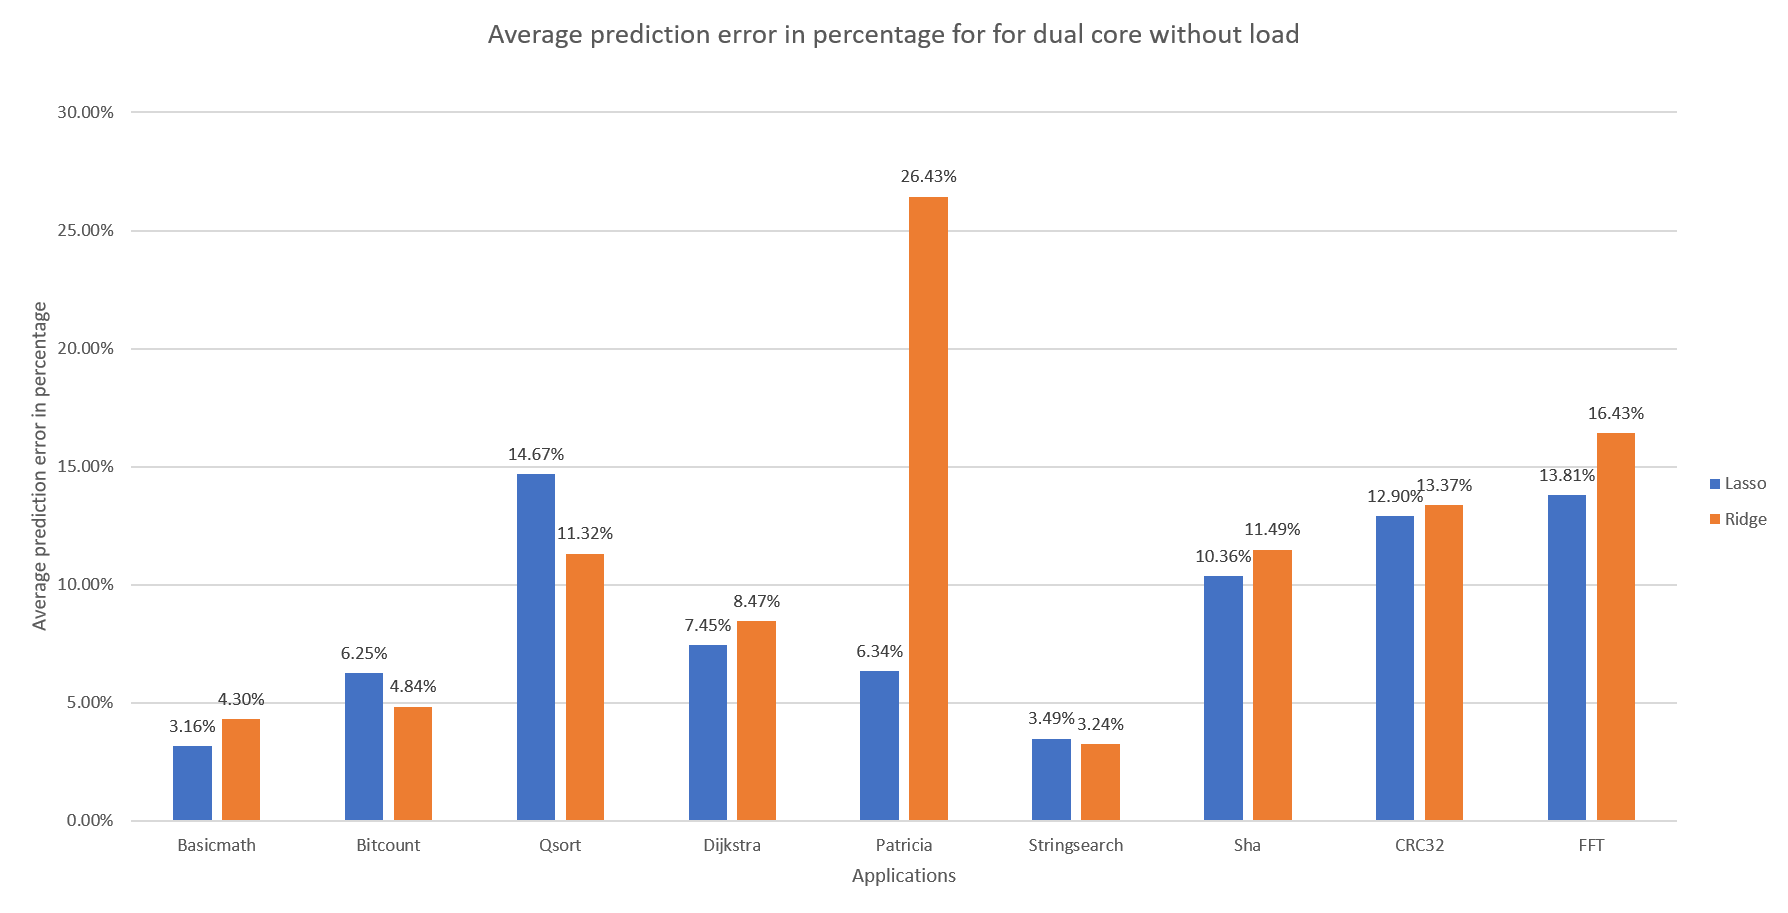
\includegraphics[width=12cm, height=8cm]{./images/result_noload}
\centering
\caption{Prediction results collected at granularity of 8000 for dual core without load}
\label{fig:r_dual_no}
\end{figure}

\subsection{Dual Core with Full Load}
Following figure \ref{fig:r_dual_full} shows the results for dual core with load scenarios at granularity of 5000 for new applications. Both training data and input data from new applications are collected at same granularity that is 5000 on dual core with full load.

\begin{figure}[h!]
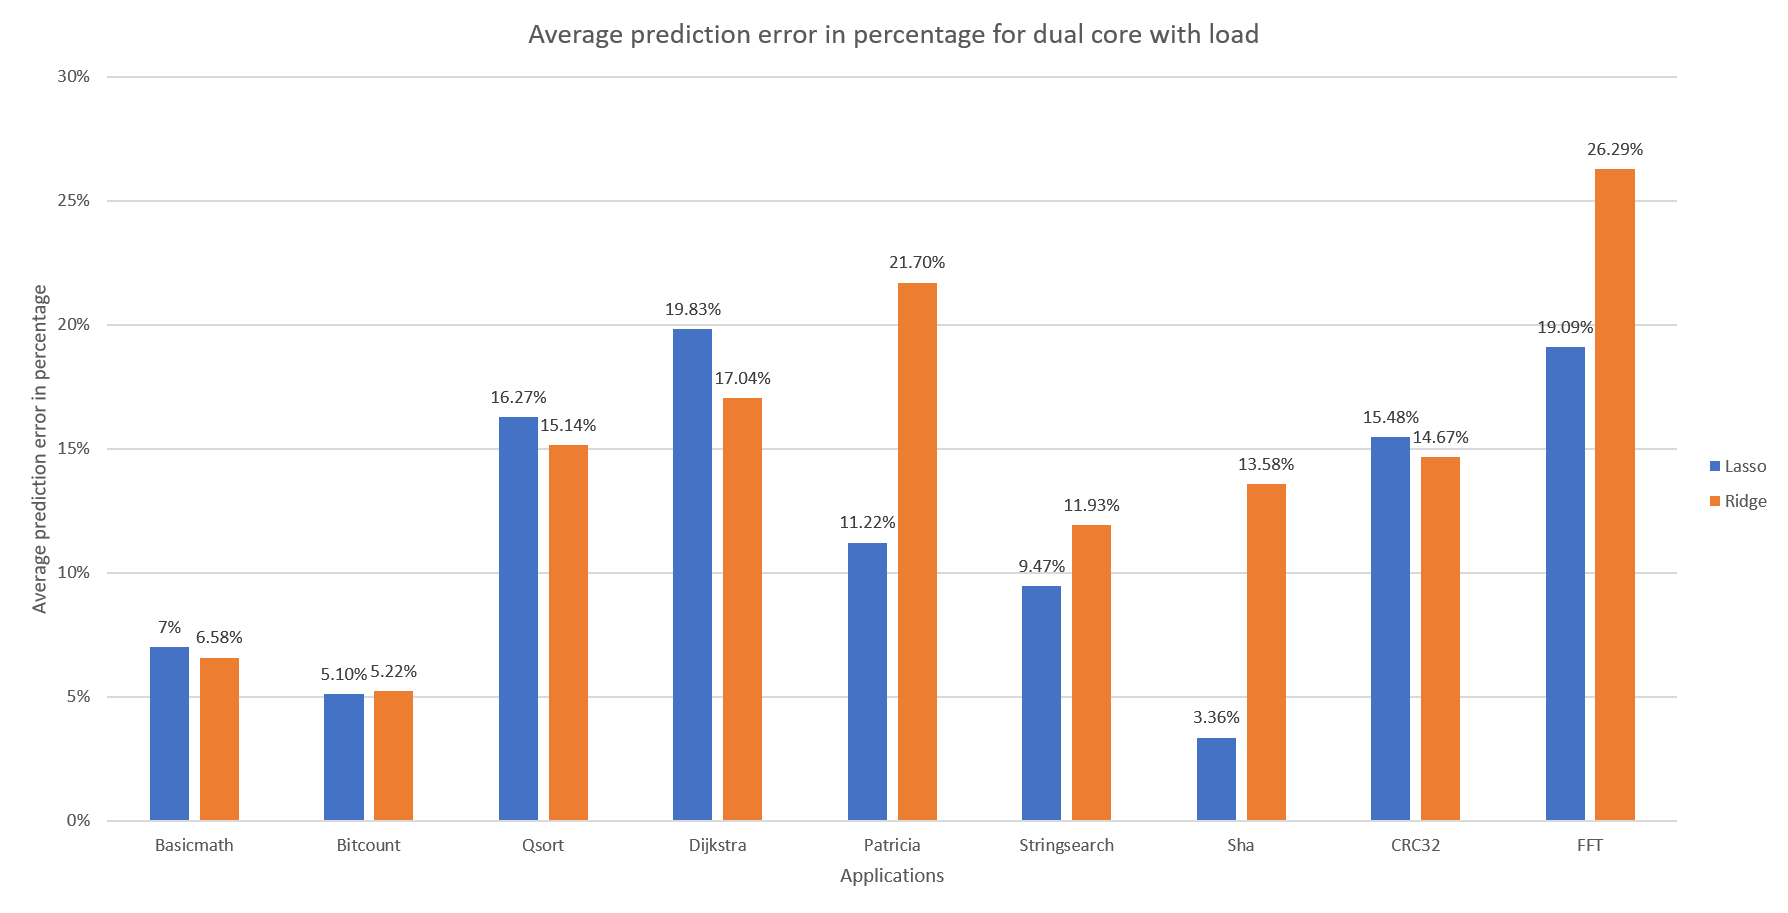
\includegraphics[width=12cm, height=8cm]{./images/result_fullload}
\centering
\caption{Prediction results collected at granularity of 5000 for dual core with full load}
\label{fig:r_dual_full}
\end{figure}

\section{Phase Granularity Tradeoffs}
We collected the training data at different granularities for single core and dual core with both scenarios. We applied cross validation on every granularity to validate machine learning algorithms.  To predict the results, we collected input data for learning algorithm also at different granularities.  But there is trade off between granularity and accuracy. We are going to see the trade off between them. 

\subsection{Single Core}
Following figure \ref{fig:td_single} shows the trade off between average prediction accuracy and granularity. We can see that initially average accuracy is low but increases with granularity and again reduces at the higher granularity. 

\begin{figure}[h!]
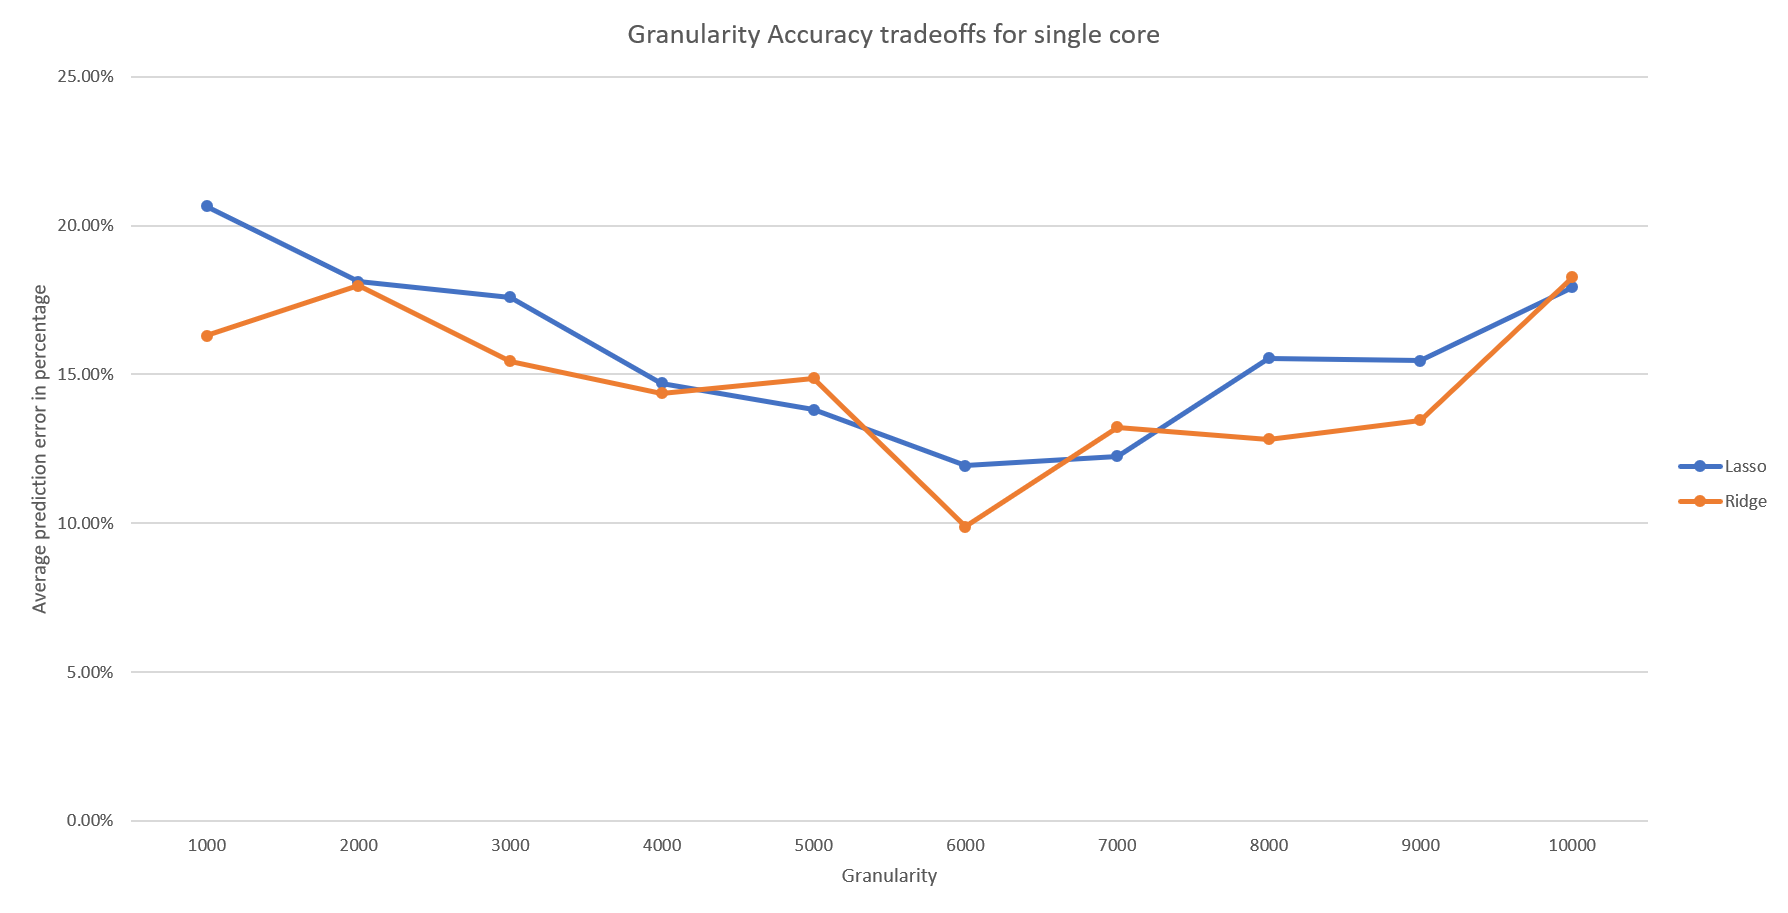
\includegraphics[width=12cm, height=8cm]{./images/td_single}
\centering
\caption{Tradeoff between granularity and accuracy of single core}
\label{fig:td_single}
\end{figure}

\subsection{Dual Core with No Load}
Following figure \ref{fig:td_noload} shows the trade off between average accuracy and granularity for dual core without load scenario. We can see variation in average accuracy but initially accuracy is low as compared in middle stages where higher accuracy can be observed. And accuracy goes low as granularity increases further. 


\begin{figure}[h!]
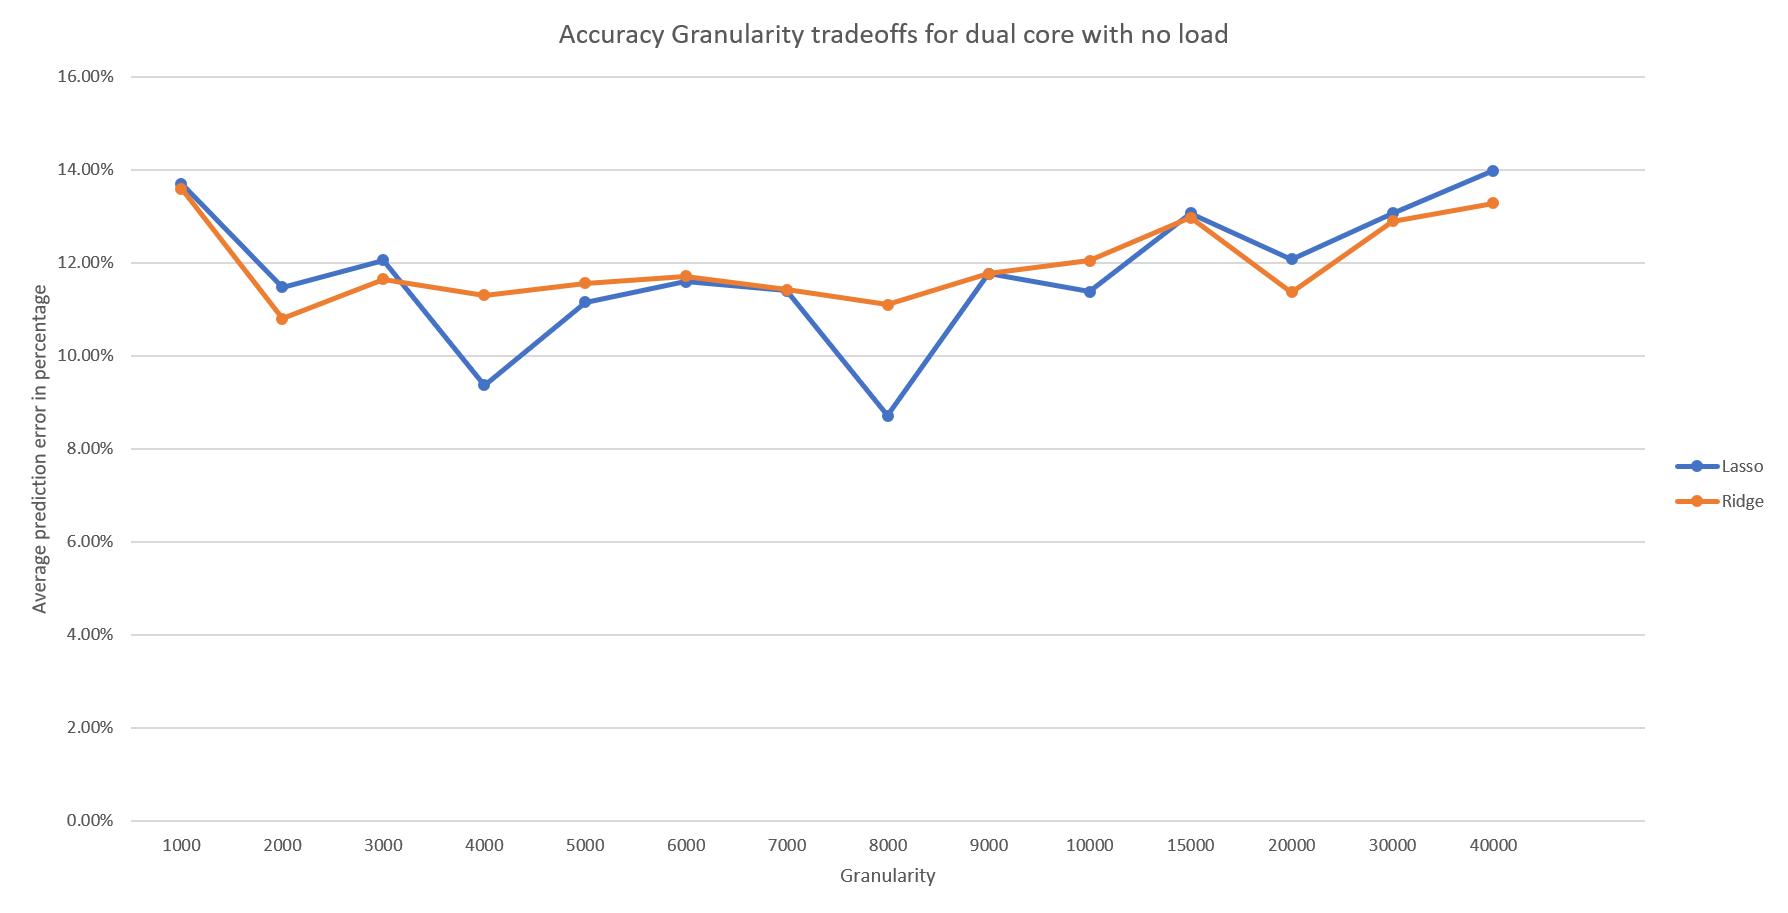
\includegraphics[width=12cm, height=8cm]{./images/td_noload}
\centering
\caption{Tradeoff between granularity and accuracy of dual core with no load}
\label{fig:td_noload}
\end{figure}

\subsection{Dual Core with Full Load}
Following figure \ref{fig:td_fullload} illustrate the accuracy and granularity tradeoff for dual core with full load scenario. We can see average accuracy is low at initial values of granularity but average accuarcy increases and remain consistent as granularity increases. As further granularity increases the average accuracy reduces. 

\begin{figure}[h!]
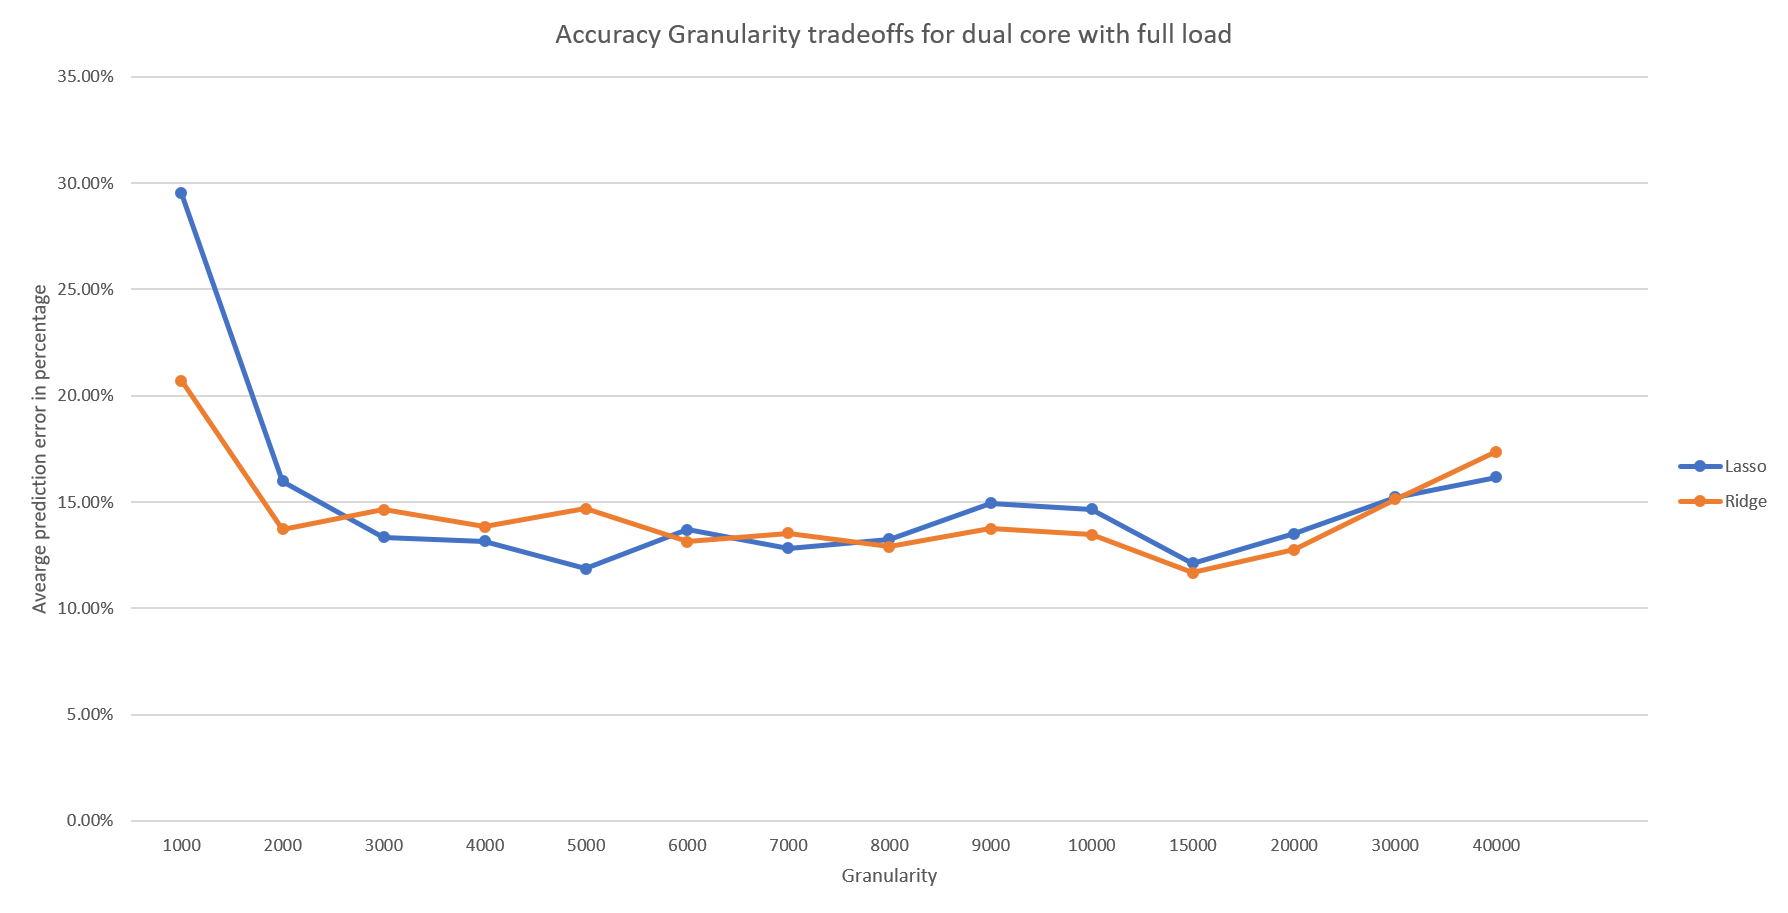
\includegraphics[width=12cm, height=8cm]{./images/td_fullload}
\centering
\caption{Tradeoff between granularity and accuracy of dual core with full load}
\label{fig:td_fullload}
\end{figure}

\subsection{Tradeoff between speed and granularity}
We collected results and training data at different values of granularities. We saw trade off between accuracy and granularity.  But size of granularity increases the number of basic blocks per phase increases and number of phases get reduced. Which causes reduction in size of data at higher granularities. For machine learning algorithm get reduced size of input as well as training data is size is lower as compare to lower granularity which causes to change in speed. As granularity size increases the prediction speed also increases. 